\begin{abstract}
We present FireRed-OCR, a systematic framework to specialize general VLMs into high-performance OCR models. Large Vision-Language Models (VLMs) have demonstrated impressive general capabilities but frequently suffer from "structural hallucination" when processing complex documents, limiting their utility in industrial OCR applications. In this paper, we introduce FireRed-OCR, a novel framework designed to transform general-purpose VLMs (based on Qwen3-VL) into pixel-precise structural document parsing experts. To address the scarcity of high-quality structured data, we construct a "Geometry + Semantics" Data Factory. Unlike traditional random sampling, our pipeline leverages geometric feature clustering and multi-dimensional tagging to synthesize and curate a highly balanced dataset, effectively handling long-tail layouts and rare document types. Furthermore, we propose a Three-Stage Progressive Training strategy that guides the model from pixel-level perception to logical structure generation. This curriculum includes: (1) Multi-task Pre-alignment to ground the model’s understanding of document structure; (2) Specialized SFT for standardizing full-image Markdown output; and (3) Format-Constrained Group Relative Policy Optimization (GRPO), which utilizes reinforcement learning to enforce strict syntactic validity and structural integrity (e.g., table closure, formula syntax). Extensive evaluations on OmniDocBench v1.5 demonstrate that FireRed-OCR achieves state-of-the-art performance with an overall score of 92.94\%, significantly outperforming strong baselines such as DeepSeek-OCR 2 and OCRVerse across text, formula, table, and reading order metrics. We open-source our code and model weights to facilitate the "General VLM to Specialized Structural Expert" paradigm.


\end{abstract}



\begin{figure}[b]
  \centering
  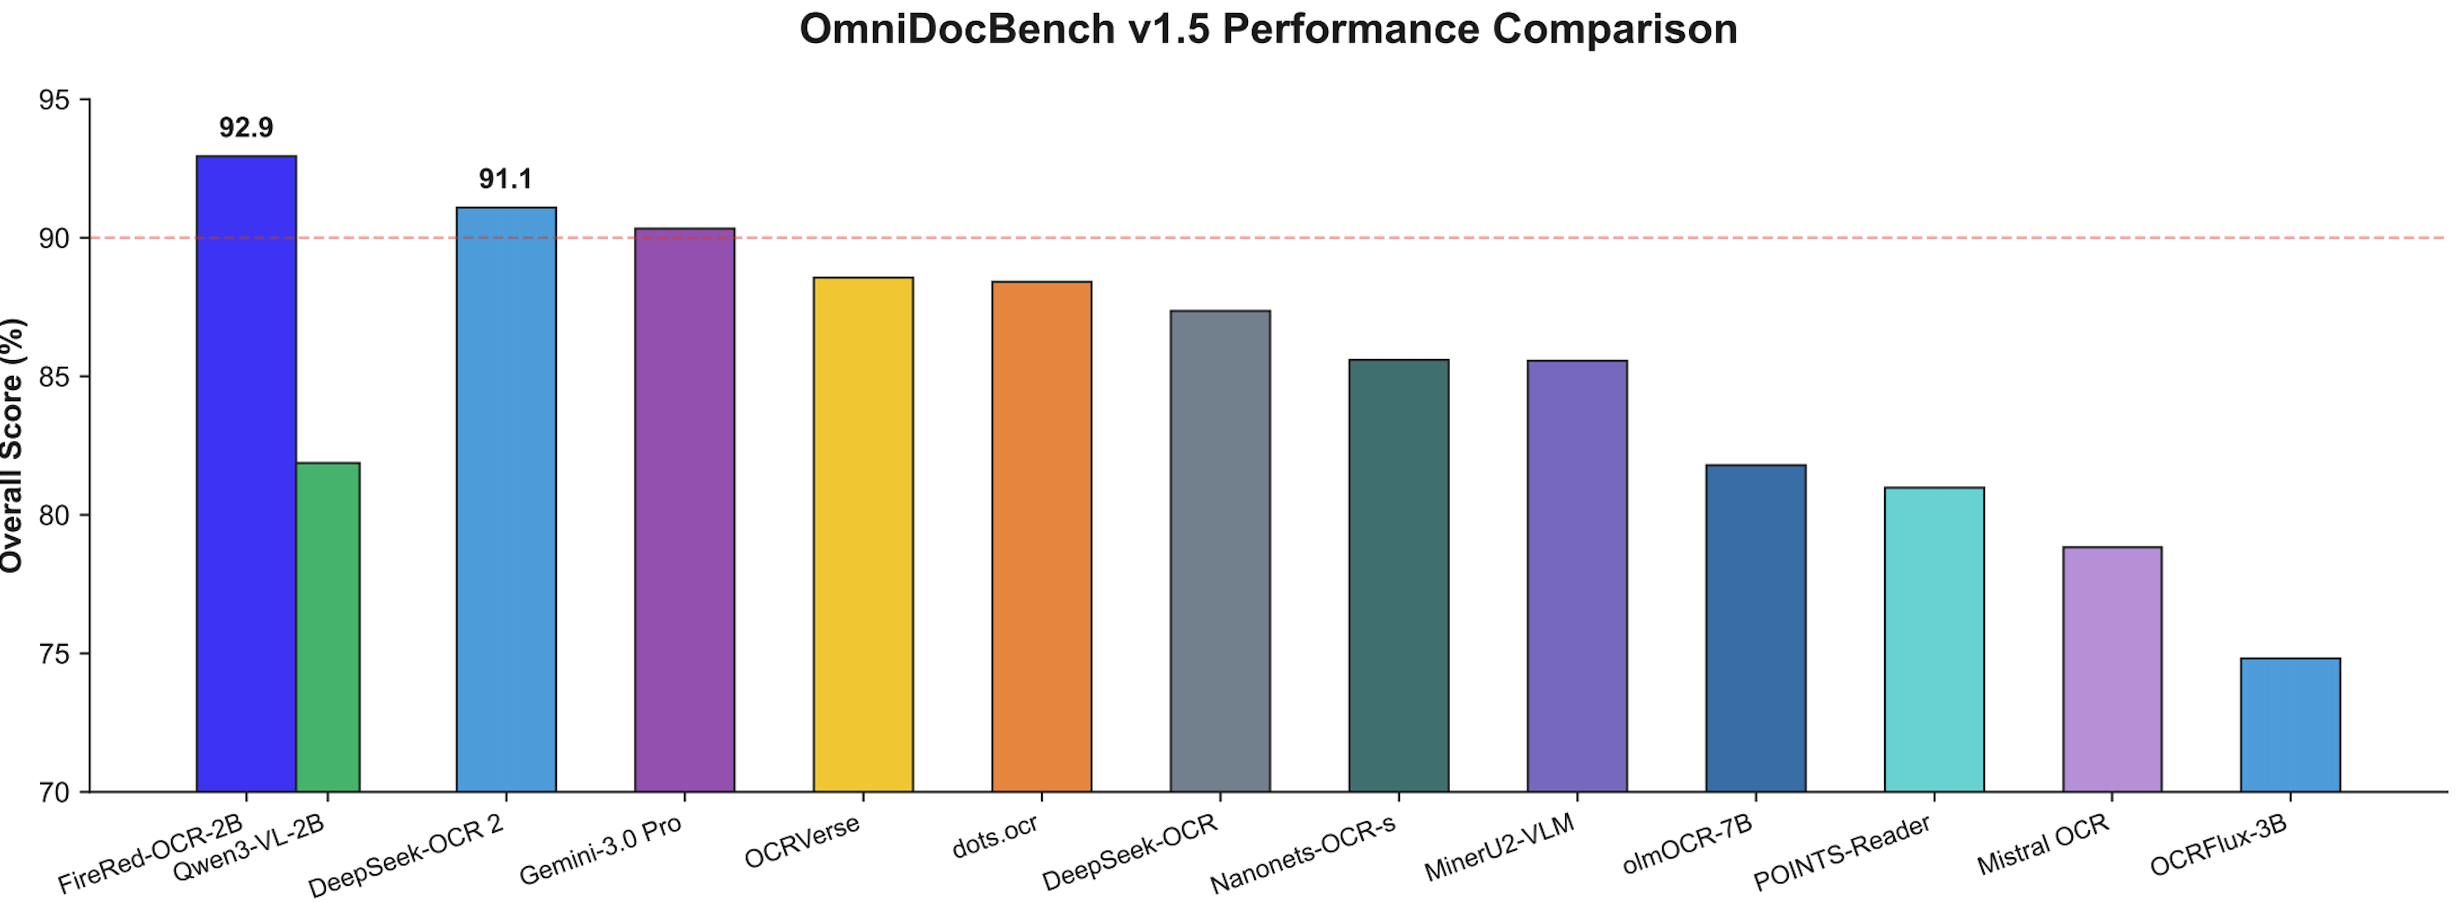
\includegraphics[width=0.9\textwidth]{figures/omnidoc_228_1.png}
  \caption{Performance comparison on the OmniDocBench v1.5 benchmark. FireRed-OCR achieves state-of-the-art performance, securing the top rank in the overall evaluation with a score exceeding 90\%.}
  \label{fig:introduction_benchmark}
\end{figure}

